%%% LaTeX Template: Article/Thesis/etc. with colored headings and special fonts
%%%
%%% Source: http://www.howtotex.com/
%%% Feel free to distribute this template, but please keep to referal to http://www.howtotex.com/ here.
%%% February 2011
%%%
%%% Modified January 2016 by CDM

%%%  Preamble
\documentclass[11pt,letterpaper]{article}
\usepackage[margin=1.0in]{geometry}
\usepackage[T1]{fontenc}
\usepackage[bitstream-charter]{mathdesign}
\usepackage[latin1]{inputenc}					
\usepackage{amsmath}						
\usepackage{xcolor}
\usepackage{cite}
\usepackage{hyphenat}
\usepackage{graphicx}
\usepackage{float}
\usepackage{subfigure}
\usepackage{sectsty}
\usepackage[compact]{titlesec} 
\usepackage[tablegrid]{vhistory}
\usepackage{pbox}
\allsectionsfont{\color{accentcolor}\scshape\selectfont}

%%% Definitions
\definecolor{accentcolor}{rgb}{0.0,0.0,0.5} 
\newcommand{\teamname}{Robo Crew}
\newcommand{\productname}{RV8 Workcell}
\newcommand{\coursename}{CSE 4316: Senior Design I}
\newcommand{\semester}{Fall 2023}
\newcommand{\docname}{Architectural Design Specification}
\newcommand{\department}{Department of Computer Science \& Engineering}
\newcommand{\university}{The University of Texas at Arlington}
\newcommand{\authors}{Akshay Paluri \\ Ameen Mahouch \\ Muhammad Anas \\ Hyun Ho Kim\\ Kundan Singh Mahato}

%%% Headers and footers
\usepackage{fancyhdr}
	\pagestyle{fancy}						% Enabling the custom headers/footers
\usepackage{lastpage}	
	% Header (empty)
	\lhead{}
	\chead{}
	\rhead{}
	% Footer
	\lfoot{\footnotesize \teamname \ - \semester}
	\cfoot{}
	\rfoot{\footnotesize page \thepage\ of \pageref{LastPage}}	% "Page 1 of 2"
	\renewcommand{\headrulewidth}{0.0pt}
	\renewcommand{\footrulewidth}{0.4pt}

%%% Change the abstract environment
\usepackage[runin]{abstract}			% runin option for a run-in title
%\setlength\absleftindent{30pt}			% left margin
%\setlength\absrightindent{30pt}		% right margin
\abslabeldelim{\quad}	
\setlength{\abstitleskip}{-10pt}
\renewcommand{\abstractname}{}
\renewcommand{\abstracttextfont}{\color{accentcolor} \small \slshape}	% slanted text

%%% Start of the document
\begin{document}

%%% Cover sheet
{\centering \huge \color{accentcolor} \sc \textbf{\department \\ \university} \par}
\vspace{1 in}
{\centering \huge \color{accentcolor} \sc \textbf{\docname \\ \coursename \\ \semester} \par}
\vspace{0.5 in}
\begin{figure}[h!]
	\centering
   	
\includegraphics[width=0.60\textwidth]{images/robocrew.jpg}
\end{figure}
\vspace{0.5 in}
{\centering \huge \color{accentcolor} \sc \textbf{\teamname \\ \productname} \par}
\vspace{0.5 in}
{\centering \large \sc \textbf{\authors} \par}
\newpage


%\vspace{1 in}
%\centerline{January 13th, 2012}
%\newpage

%%% Revision History
\begin{versionhistory}
  	\vhEntry{0.1}{11.06.2023}{AM, MA, AP, HK, KM}{document creation}
\end{versionhistory}
\newpage

%%% Table of contents
\setcounter{tocdepth}{2}
\tableofcontents
\newpage

%%% List of figures and tables (optional)
\listoffigures
\listoftables
\newpage

%%% Document sections
\section{Introduction}
This product is a high level working prototype of an industrial level robot which serves the purpose of ordering and arranging the boxes by scanning the QR codes. The boxes will be picked by a gripper (custom designed) and will be sorted. The robot arm is connected to a PLC controller and the arm is set on to an additional axis (i.e. linear rail) which is also connected to a servo amplifier present in the PLC. This PLC controller is connected to a PC containing various software to control the robot arm. Raspberry Pi is used for the QR code detection and decision making which is connected to a camera.
\newpage
\section{System Overview}
This section defines the top-level logical view of the design and describes the detail architectural strategy for the RV8 work cell system flow. Three separate layers make up the structure of the system: input, processing, and output. With the help of these layers, which are all essential to the system, the robot is able to carry out dynamic tasks that are dependent on the processing of sensor data. A high-level block diagram that shows the connections and interactions between different layers is included in this part to provide readers a thorough understanding of the architecture of the entire system. A robotic system's input layer, which makes use of sensors like a gate sensor and an E-stop is essential for task execution. E-stops offer an emergency shutdown signal that allows the system to be stopped right away. The robot arm's speed is controlled by the Gate sensor, which also communicates with the controller to find out the cage gate's present state. Efficiency and safety are prioritized in this design, which allows the robot to respond and adapt to a variety of scenarios while integrating security features like gate status monitoring and emergency stops. With the integration of sensors will perform the operation such as splashing multi-color paint to the desire target with great level of precision. PC and the trigger switch will be inter-connected to the PC to perform the necessary communication to perform the given task.  

\begin{figure}[h!]
	\centering
 	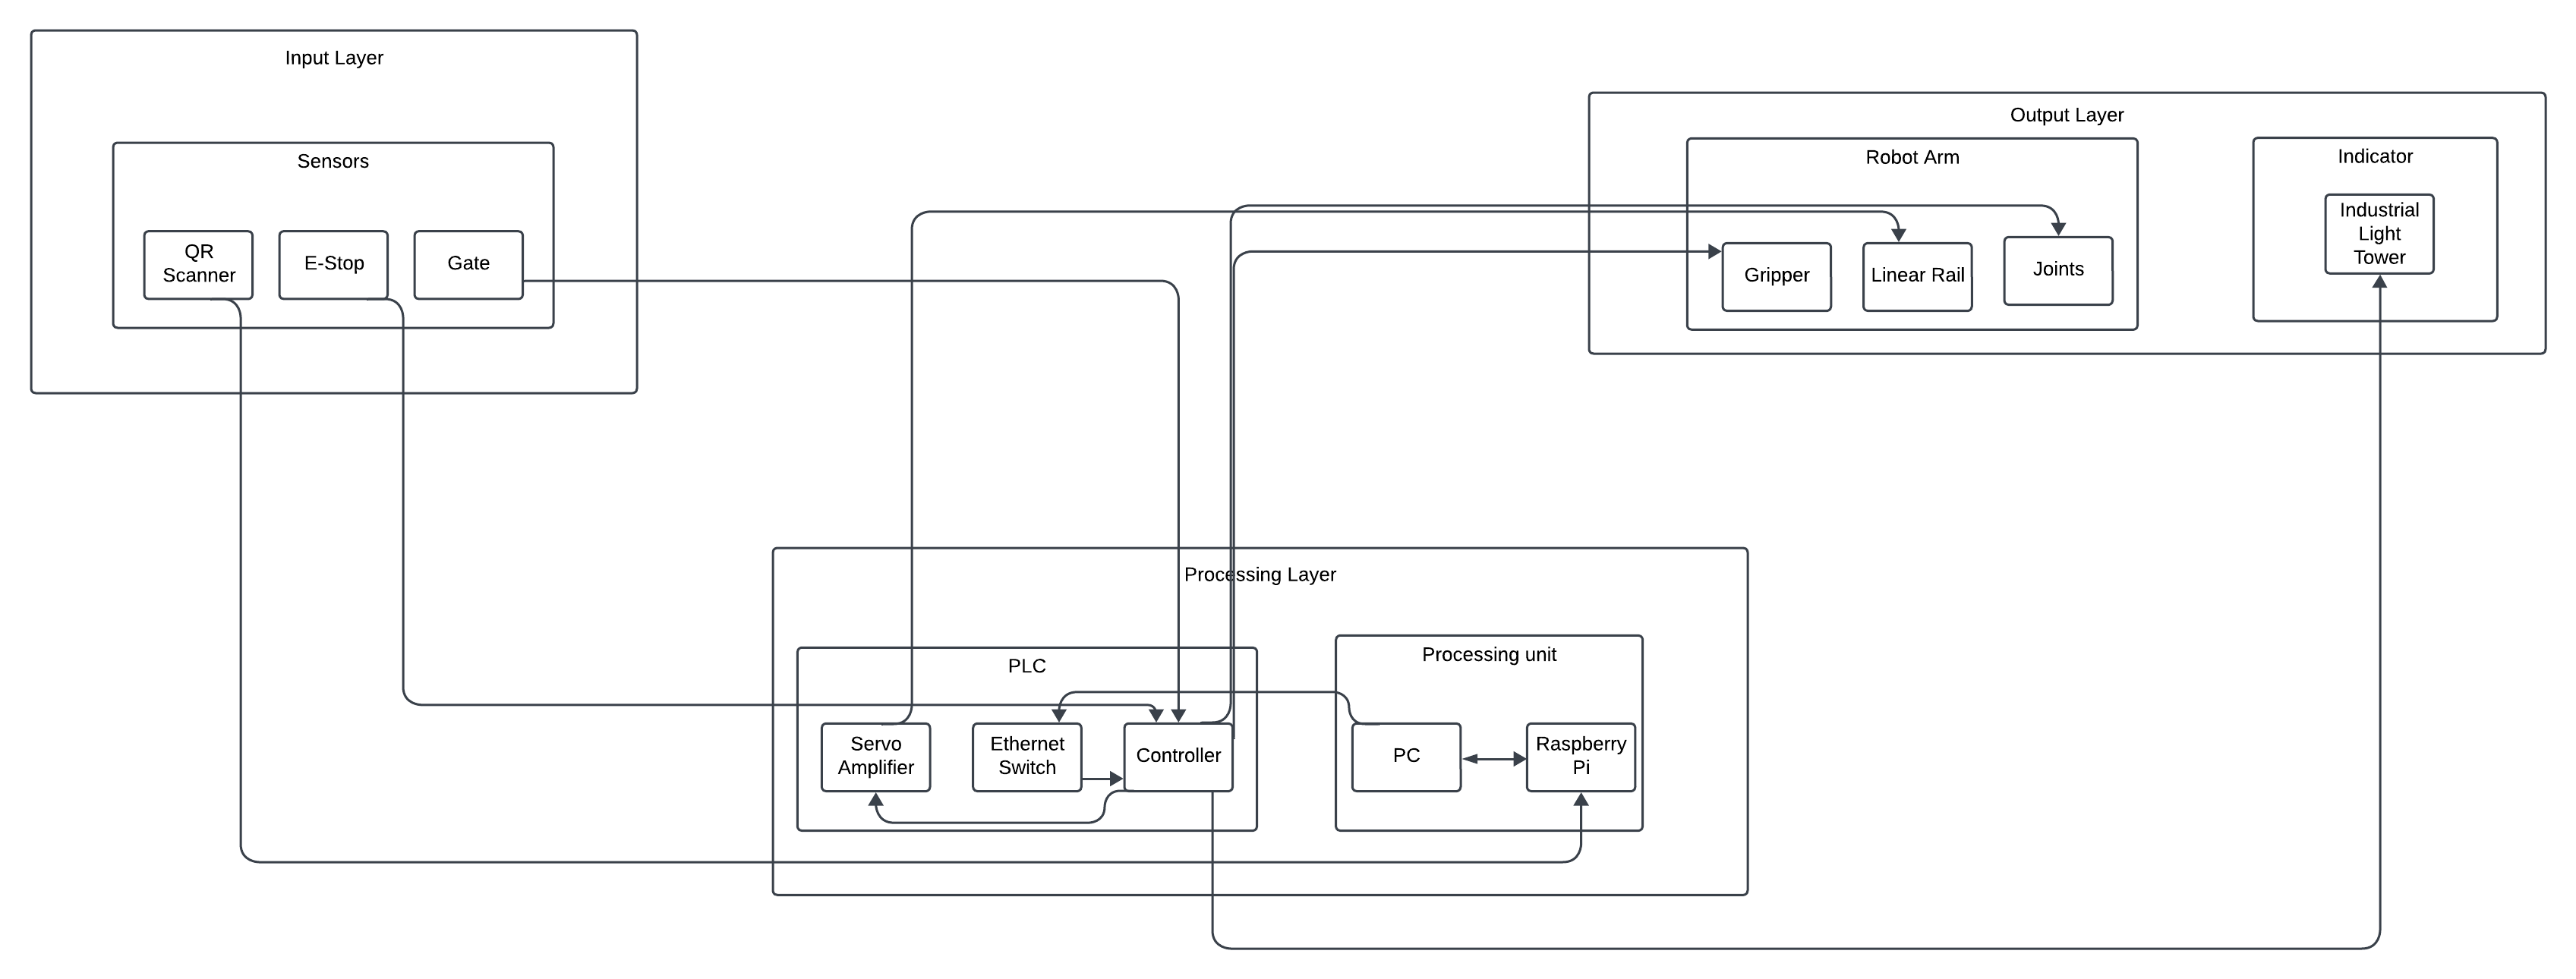
\includegraphics[width=1\textwidth]{images/system_subystem.png}
 \caption{System architecture}
\end{figure}

\newpage
\section{Subsystem Definitions \& Data Flow}
This section breaks down your layer abstraction to another level of detail. Here you grapically represent the logical subsytems that compose each layer and show the interactions/interfaces between those subsystems. A subsystem can be thought of as a programming unit that implements one of the major functions of the layer. It, therefore, has data elements that serve as source/sinks for other subsystems. The logical data elements that flow between subsystems need to be explicitly defined at this point, beginning with a data flow-like diagram based on the block diagram.

\begin{figure}[h!]
	\centering
 	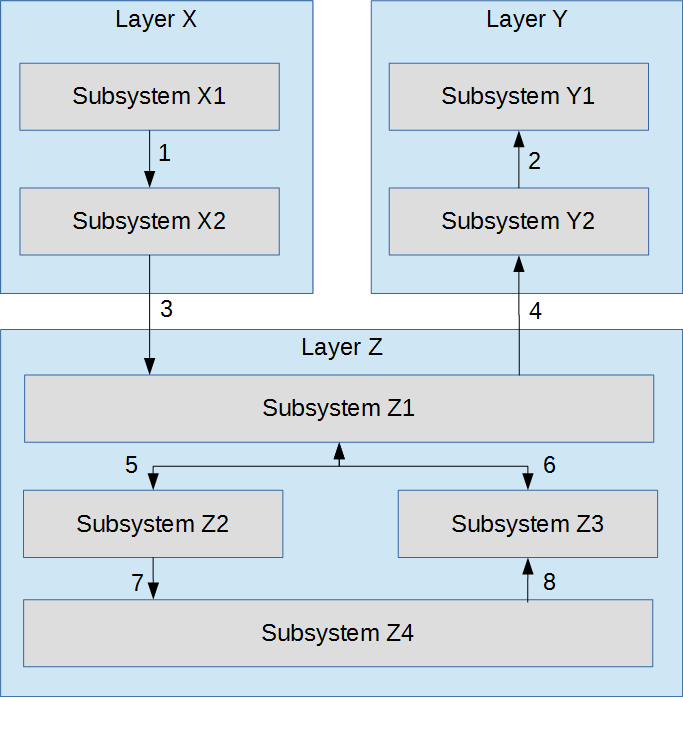
\includegraphics[width=\textwidth]{images/data_flow}
 \caption{A simple data flow diagram}
\end{figure}

\newpage
\newpage
\section{Input Layer Subsystems}
The input layer is comprised of various sensors, such as the E-stop switch and inductive limit switches. The input layer receives these inputs and directs them to the programmable logic controller for further processing. The host PC is also a component within the input layer, in charge of programming and writing to the system. We can configure the robot arm and the linear rail to execute a task, and in case of an emergency, the E-stop can halt our program instantly.


\subsection{Host PC}
The host PC acts as the centralized component for communication between the robot arm and the PLC. Comprised of software like RTToolbox and GXWorks3, the PC can program the different subsystems to accomplish the application task.

\begin{figure}[h!]
	\centering
 	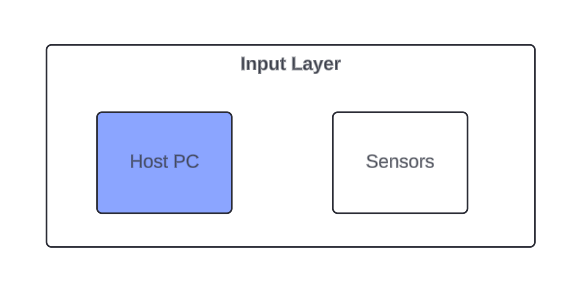
\includegraphics[width=0.60\textwidth]{images/Input_Host.png}
 \caption{Host PC subsystem description diagram.}
\end{figure}

\subsubsection{Assumptions}
Host PC contains all the required software to program the movement of the robot. The program written in host PC will act as an input for our system. 


\subsubsection{Responsibilities}
The program will contain logic behind the specific movement of the robot. The program will be written in a way that the robot only performs a fixed task.


\subsubsection{Subsystem Interfaces}
\begin {table}[H]
\caption {Subsystem interfaces} 
\begin{center}
    \begin{tabular}{ | p{1cm} | p{6cm} | p{3cm} | p{3cm} |}
    \hline
    ID & Description & Inputs & Outputs \\ \hline
    \#01 & Write a robot movement program & \pbox{3cm}{-} & \pbox{3cm}{sends program}  \\ \hline
    \#02 & Write a logic program & \pbox{3cm}{-} & \pbox{3cm}{sends program}  \\ \hline
    \end{tabular}
\end{center}
\end{table}

\subsection{Sensors}
The sensors subsystem consists of emergency stops and inductive limit switches. E-stops serve as a safety feature, allowing users to halt the robot in the event of unexpected actions or when they desire. This sensor can stop the program, regardless of the current processing state. The inductive limit switches act as motion boundaries for the robot and aid with calibration.

\begin{figure}[h!]
	\centering
 	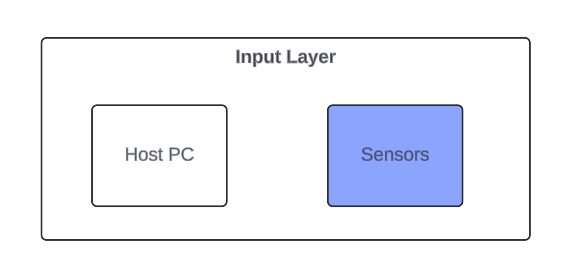
\includegraphics[width=0.60\textwidth]{images/Input_Snsors.png}
 \caption{Sensors subsystem description diagram}
\end{figure}

\subsubsection{Assumptions}
E-stops can be pressed to immediately stop the robot in case of potential collisions, unexpected behavior, or excessive temperature increases. The emergency stops are used in emergency situations, and are not the normal standard for halting robot movement. The inductive limit switches send signals to the robot controller to indicate the robot is reaching its boundary limits. The program written by the PC must include a dynamic calibration sequence that references these limits.

\subsubsection{Responsibilities}
If users press any of the E-stops, the system stops by transmitting the changed input value to the controller. When any of the emergency stop switches are pressed, the switch is closed and the electric signal is outputted, and this value is then relayed to the controller to halt the system. Similarly, any time the robot travels over the limit switch, the contact is closed and sends a signal to the PLC.

\subsubsection{Subsystem Interfaces}

\begin {table}[H]
\caption {Subsystem interfaces} 
\begin{center}
    \begin{tabular}{ | p{1cm} | p{6cm} | p{3cm} | p{3cm} |}
    \hline
    ID & Description & Inputs & Outputs \\ \hline
    \#03 & E-stop signal & \pbox{3cm}{button status} & \pbox{3cm}{closed or open}  \\ \hline
    \#04 & Inductive switches & \pbox{3cm}{closed or open} & \pbox{3cm}{0 or 1}  \\ \hline
    \end{tabular}
\end{center}
\end{table}

% \subsection{Gate}
% The gate sensor is a safety component that detects whether the gate is open or closed.

% \begin{figure}[h!]
% 	\centering
%  	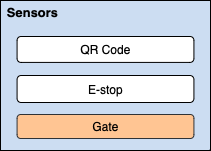
\includegraphics[width=0.60\textwidth]{images/gate.png}
%  \caption{Gate subsystem description diagram}
% \end{figure}

% \subsubsection{Assumptions}
% When the gate is open, the gate sensor sends a 'True' signal to the control, causing the robot to move slowly.

% \subsubsection{Responsibilities}
% Since the gate sensor detects value changes, it must transmit the changed value to the controller for a response.

% \subsubsection{Subsystem Interfaces}
% \begin {table}[H]
% \caption {Subsystem interfaces} 
% \begin{center}
%     \begin{tabular}{ | p{1cm} | p{6cm} | p{3cm} | p{3cm} |}
%     \hline
%     ID & Description & Inputs & Outputs \\ \hline
%     \#03 & Gate open or close & \pbox{3cm}{gate} & \pbox{3cm}{True or False}  \\ \hline
%     \end{tabular}
% \end{center}
% \end{table}


\newpage
\section{Processing Layer Subsystems}
In this section, the processing unit layer is described in some detail in terms of its specific subsystems. The processing unit comprises three primary components: the PLC, the Ethernet switch, and the robotic controller. This layer plays a crucial role in the robotic system by acquiring input data from sensors and processing it before transmitting the processed data to the robotic arm and air compressor.

\subsection{PLC}
Programmable Logic Controller (PLC) is an industrial automation device used for controlling and automating various processes in manufacturing, production and other industrial applications.

\begin{figure}[h!]
	\centering
 	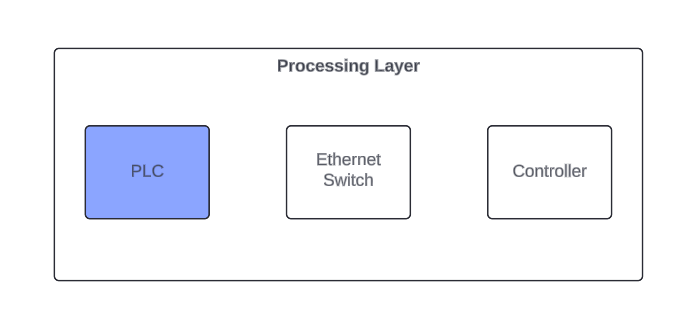
\includegraphics[width=0.60\textwidth]{images/Processing_PLC.png}
 \caption{PLC subsystem.}
\end{figure}

\subsubsection{Assumptions}
PLC is like a central processing unit of this product. The input comes from the input layer and is written onto to the PLC since the primary purpose of using a PLC is to automate the process. 

\subsubsection{Responsibilities}
The responsibility of the PLC being used in this project is to save the logical program and movement program, and to continuously process the state of the work cell. The PLC is written with a logic-based program that receives input signals from the input layer and manipulates them according to the program specification. PLC is also responsible to send output signals to other components within the system such as the air compressor and light tower to conclude the process. The output signals are computed via the logic written in the PLC. It also receives input signals from inductive switches for calibration purposes. 


\begin {table}[H]
\caption {Subsystem interfaces} 
\begin{center}
    \begin{tabular}{ | p{1cm} | p{4cm} | p{4cm} | p{4cm} |}
    \hline
    ID & Description & Inputs & Outputs \\ \hline
    \#01 & Programmable Logic Controller & \pbox{4cm}{Logic Program} & \pbox{4cm}{Send to different devices}  \\ \hline
    \#02 & Programmable Logic Controller & \pbox{4cm}{Movement Program} & \pbox{4cm}{Send to Controller}
    \\\hline
    \#03 & Programmable Logic Controller & \pbox{4cm}{Inductive switches} & \pbox{4cm}{Light Tower}\\
    \hline
    \end{tabular}
\end{center}
\end{table}


\newpage
%\section{Processing Unit Layer Subsystems}
\subsection{Ethernet Switch}
The Ethernet switch bridges communication between 3 crucial components: the host PC, the robot controller, and the PLC. The Ethernet switch is located within the control cabinet and insures consistent and instantaneous communication over the network.
\begin{figure}[h!]
	\centering
 	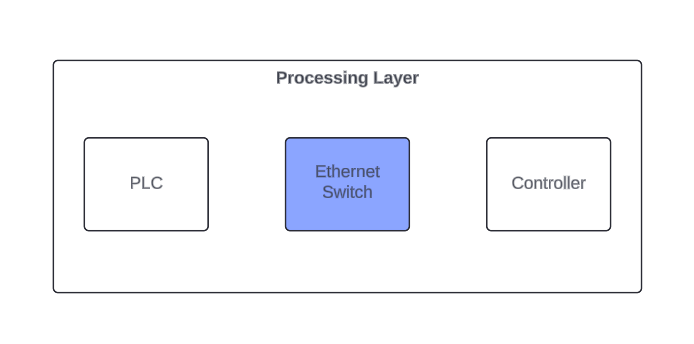
\includegraphics[width=0.60\textwidth]{images/Processing_Ethernet.png}
 \caption{Ethernet subsystem}
\end{figure}

\subsubsection{Assumptions}
A stable Ethernet connection is assumed for consistent data transfer. The components are configured to be on the same sub-network to communicate. Additionally, the robot controller and PLC must be configured with Mitsubishi's CC-Link IE Field Network to ensure signal transfer.
\subsubsection{Responsibilities}
The Ethernet switch is responsible for routing and forwarding data packets between the robot controller, PLC, and other networked devices. The switch must be consistent to ensure precision and fast transmission. Without the Ethernet switch, the robotic work cell cannot function properly and errors will arise from a lack of communication.

\subsubsection{Subsystem Interfaces}

\begin {table}[H]
\caption {Subsystem interfaces} 
\begin{center}
    \begin{tabular}{ | p{1cm} | p{6cm} | p{4cm} | p{5cm} |}
    \hline
    ID & Description & Inputs & Outputs \\ \hline
    \#04 & Data input from PC & \pbox{4cm}{CAT6 Ethernet Cable} & \pbox{5cm}{CC-Link processed packets}  \\ \hline
    \#05 & Data input from PLC & \pbox{4cm}{CAT6 Ethernet Cable} & \pbox{5cm}{CC-Link processed packets}  \\ \hline
    \#06 & Data input from CR-800 Controller & \pbox{4cm}{CAT6 Ethernet Cable} & \pbox{5cm}{CC-Link processed packets}  \\ \hline

    \end{tabular}
\end{center}
\end{table}

\subsection{Controller}
Controllers are designed to seamlessly integrate with robots. These sophisticated devices serve as the brain of robots, governing their actions and enabling precise control.
%The Raspberry Pi serves as an integral component of the processing unit within the robot system. It fulfills the role of an edge computing device, responsible for initial data processing and interfacing between the sensors and the host PC. Specifically, the Raspberry Pi is responsible for collecting data from a variety of sensors, including those for QR code scanning and other environmental monitoring.
\begin{figure}[h!]
	\centering
 	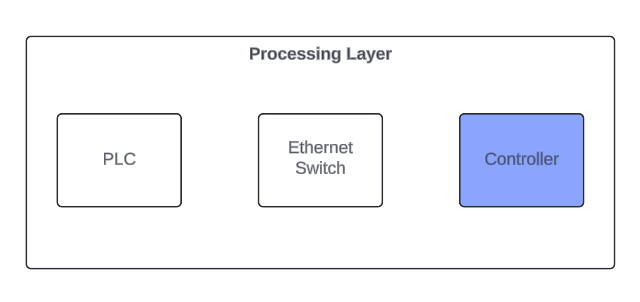
\includegraphics[width=0.60\textwidth]{images/Processsing_controller.png}
 \caption{Controller subsytem}
\end{figure}

\subsubsection{Assumptions}
The primary role of a robot controller is to receive instructions from a PLC and external sensors.

    
\subsubsection{Responsibilities}
Responsibilities of controller is to precisely manipulate the robot's joints according to a specific sequence or pattern. In addition, it also receives signals from E-stops which halts the robot functionality.

\subsubsection{Subsystem Interfaces}

\begin {table}[H]
\caption {Subsystem interfaces} 
\begin{center}
    \begin{tabular}{ | p{1cm} | p{6cm} | p{4cm} | p{5cm} |}
    \hline
    ID & Description & Inputs & Outputs \\ \hline
    \#07 & Controller & \pbox{4cm}{signals} & \pbox{5cm}{movement of joints}  \\ \hline
    \#08 & Controller & \pbox{4cm}{Emergency stops} & \pbox{5cm}{Halting the robot movement}  \\ \hline
    \end{tabular}
\end{center}
\end{table}



\newpage
\newpage
\section{Robot Arm Layer Subsystems}
This section talks about the layer of the robot arm and how each components are going to interact with necessary data inputs to perform the task of palletizing and depalletizing the boxes. The primary goal of this layer is to interact with the boxes and configure the necessary position the arm needs to be in to execute the task.
\begin{figure}[h!]
	\centering
 	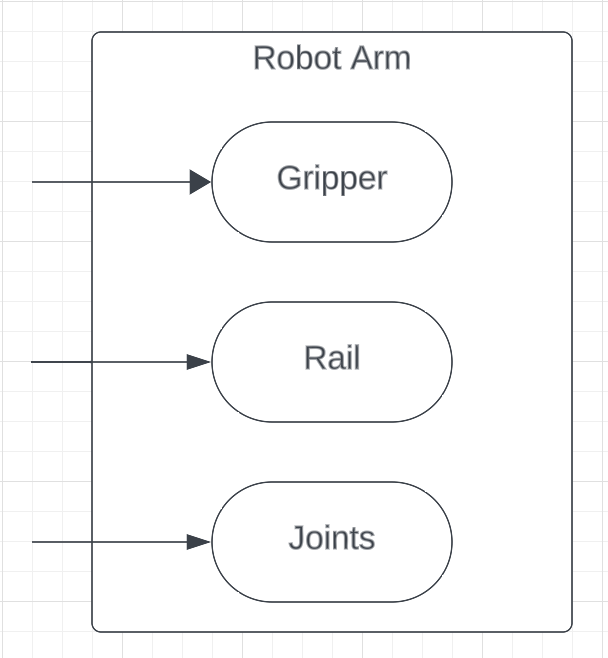
\includegraphics[width=0.60\textwidth]{images/arm}
 \caption{Robot Arm diagram}
\end{figure}


\subsection{Gripper}
This layer consists of the gripper which primarily requires the use of the hydraulic suction to create or remove grip to the boxes.

\begin{figure}[h!]
	\centering
 	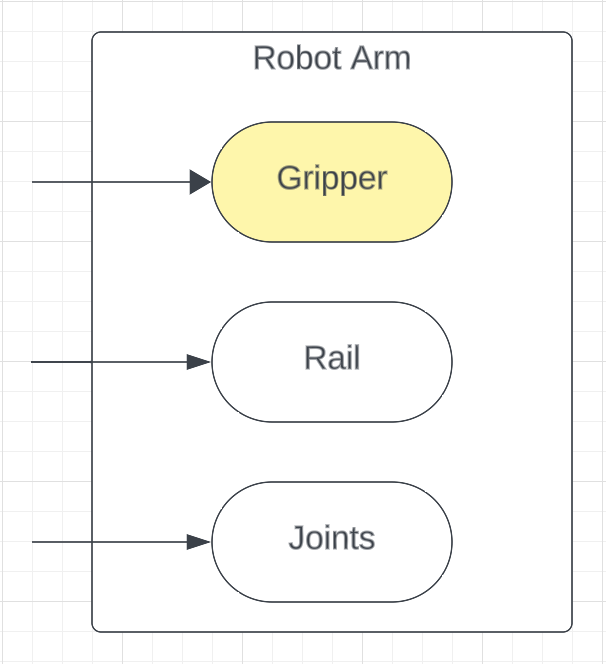
\includegraphics[width=0.60\textwidth]{images/gripper.png}
 \caption{Robot Arm diagram}
\end{figure}

\subsubsection{Assumptions}
Any wiring required for the gripper is already provided and will be stable to perform the necessary actions for the gripper to execute its task.

\subsubsection{Responsibilities}
The gripper is responsible for creating grip on to the boxes and remove any grip on to the boxes. The data to create/remove the grip comes from PLC which uses QR code to send the data to hold a grip on to the boxes and once the task is executed, the gripper is given the data to remove the hold on the boxes.

\subsubsection{Subsystem Interfaces}
\begin {table}[H]
\caption {Subsystem interfaces}
\begin{center}
    \begin{tabular}{ | p{1cm} | p{6cm} | p{3cm} | p{3cm} |}
    \hline
    ID & Description & Inputs & Outputs \\ \hline
    \#1 & Suction grip & \pbox{3cm}{Box detection} & \pbox{3cm}{hydraulic grip}  \\ \hline
    \end{tabular}
\end{center}
\end{table}

\subsection{Rail}
This layer consists of the linear rail required to give the robot arm a linear motion.

\begin{figure}[h!]
	\centering
 	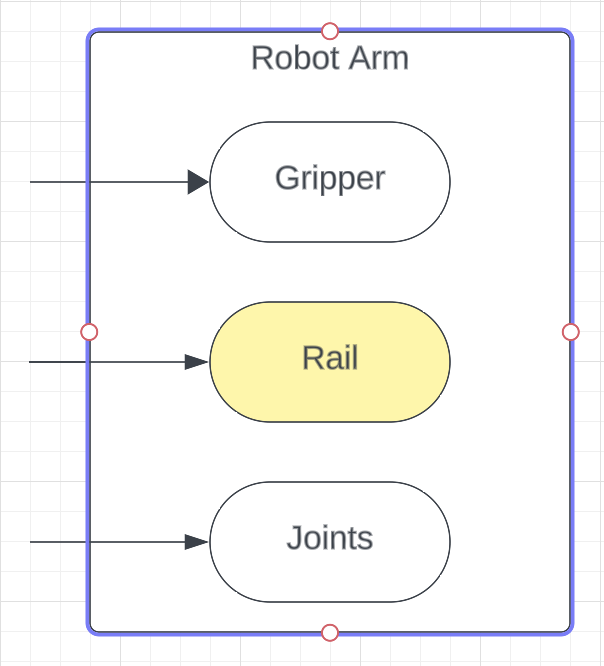
\includegraphics[width=0.60\textwidth]{images/rail.png}
 \caption{Robot Arm diagram}
\end{figure}

\subsubsection{Assumptions}
Any wiring required for the motion of linear rail is already provided and is stable when the robot arm is in motion.

\subsubsection{Responsibilities}
The linear rail is responsible for moving the entire robot arm in a linear motion in defined boundaries in order to get to a configuration to move the boxes. The linear rail will get the data from the servo amplifier which is a component of the PLC.

\subsubsection{Subsystem Interfaces}
\begin {table}[H]
\caption {Subsystem interfaces}
\begin{center}
    \begin{tabular}{ | p{1cm} | p{6cm} | p{3cm} | p{3cm} |}
    \hline
    ID & Description & Inputs & Outputs \\ \hline
    \#2 & Rail Motion & \pbox{3cm}{PLC data } & \pbox{3cm}{linear movement}  \\ \hline
    \end{tabular}
\end{center}
\end{table}


\subsection{Joints}
This layer consists of the configurations required for the arm to be able to reach the boxes.

\begin{figure}[h!]
	\centering
 	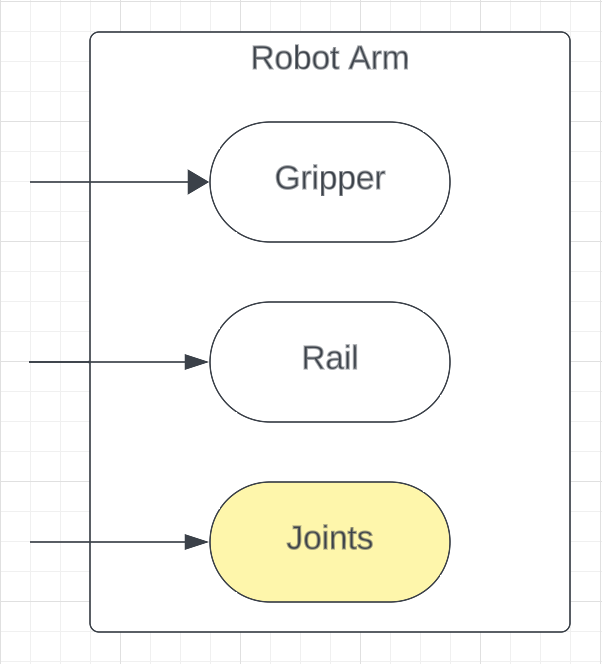
\includegraphics[width=0.60\textwidth]{images/joints.png}
 \caption{Robot Arm diagram}
\end{figure}

\subsubsection{Assumptions}
Any wiring required for the arm to be in multiple configurations is provided and would be stable while the arm is in motion.

\subsubsection{Responsibilities}
The joints are responsible for the movement of the gripper and be in a certain configuration so that the gripper is able to reach the boxes. Joints communicate directly with the PLC which gives the appropriate data to be in a certain configuration space.

\subsubsection{Subsystem Interfaces}
\begin {table}[H]
\caption {Subsystem interfaces}
\begin{center}
    \begin{tabular}{ | p{1cm} | p{6cm} | p{3cm} | p{3cm} |}
    \hline
    ID & Description & Inputs & Outputs \\ \hline
    \#2 & Joint Configuration & \pbox{3cm}{PLC data} & \pbox{3cm}{joint angle}  \\ \hline
    \end{tabular}
\end{center}
\end{table}

\newpage
\section{Indicator Layer Subsystems}
The indicator layer will be responsible for the output of the system, where the indicator subsystem consists of an industrial light tower, which displays the status of the working cell.   

\subsection{Industrial Light Tower}
An industrial light tower system, typically used in a working cell or industrial setting, serves several essential responsibilities to ensure the efficient and safe operation of the workspace. The specific responsibilities of an industrial light tower system may vary depending on the application. For our system, it serves as an inference to the work environment as it indicates different modes with colored LEDs as get input from the controller and outputs as LEDs. 
\begin{figure}[h!]
	\centering
 	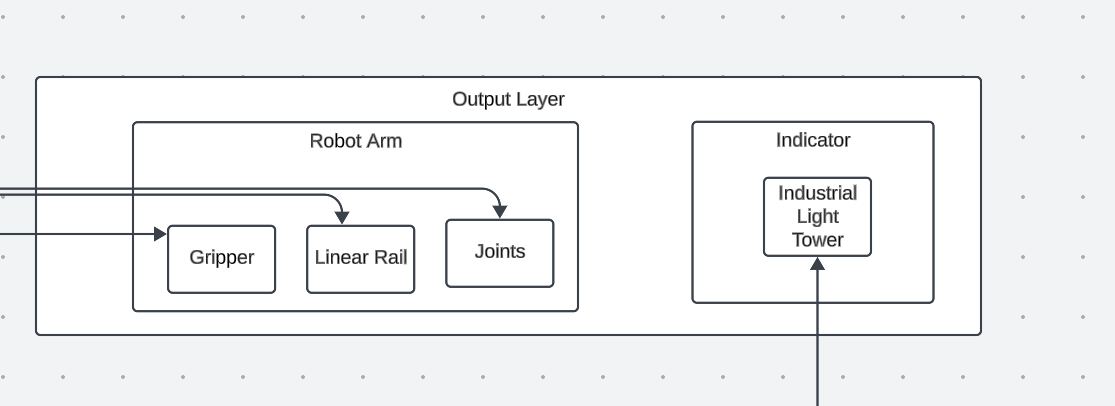
\includegraphics[width=0.60\textwidth]{images/indicator.png}
 \caption{Indicator subsystem description diagram}
\end{figure}

\subsubsection{Assumptions}
The "Indicator" subsystem assumes that it will receive status information from the Controller about the working status of the robot arm. It is assumed that this system will be a reliable communication source or interface to update the status of the working cell. 
\subsubsection{Responsibilities}
Signaling and Alerts: Industrial light tower systems often include signal lights or beacons. These lights can be used to convey information or alerts to workers or nearby personnel. Common signals include indicating when a machine is running, signaling the need for maintenance or repair, or warning of specific hazards or emergencies.

Status Indication: The light tower system can provide status indications for machines or equipment within the working cell. 

Safety: Ensuring the safety of workers is a primary responsibility. Light towers can be programmed to flash or change colors to draw attention to potential safety hazards, such as moving equipment or areas that require caution.

\subsubsection{Subsystem Interfaces}

\begin {table}[H]
\caption {Subsystem interfaces} 
\begin{center}
    \begin{tabular}{ | p{1cm} | p{6cm} | p{3cm} | p{3cm} |}
    \hline
    ID & Description & Inputs & Outputs \\ \hline
    \#01 & Stop operating & \pbox{3cm}{controller} & \pbox{3cm}{red led signal}  \\ \hline
    \#02 & Require caution & \pbox{3cm}{controller} & \pbox{3cm}{yellow led signal}  \\ \hline
    \#03 & Operating Mode & \pbox{3cm}{controller} & \pbox{3cm}{green led signal}  \\ \hline
    \end{tabular}
\end{center}
\end{table}


\newpage

%%% References
\bibliographystyle{plain}
\bibliographystyle{reference/IEEEtran_custom}
\bibliography{reference/refs}{}

\end{document}